\chapter{Implementierung Montage}
In diesem Kapitel wird auf die Implementierung aller notwendiger Softwarekomponenten eingegangen, damit im Industriedemonstrator Kugelschreiber montiert werden können. 
\section{Grundüberlegungen}
Der Roboter muss fähig sein einem Montageablauf zu folgen, um Kugelschreiber montieren zu können. Dieser wird in einem eigenen Package cell\_core implementiert. Dieses Package erzeugt die move\_group und kann Kollisionsobjekte in der Planungsszene generieren. Ein zweites Package ist für die Ansteuerung der SMC Aktuatoren zuständig. Dieses Package smc\_grippers ist die Schnittstelle zwischen der ROS-Kommunikation und der Kommunikation über EtherCAT. Für die Schnittstelle zur restlichen Anlage steht der in Abschnitt \ref{sec:SWschnittstellen} bereits erwähnte HTTP-Server zur Verfügung. Dieser befindet sich im Package http\_server.
\begin{figure}[H]
	\centering
	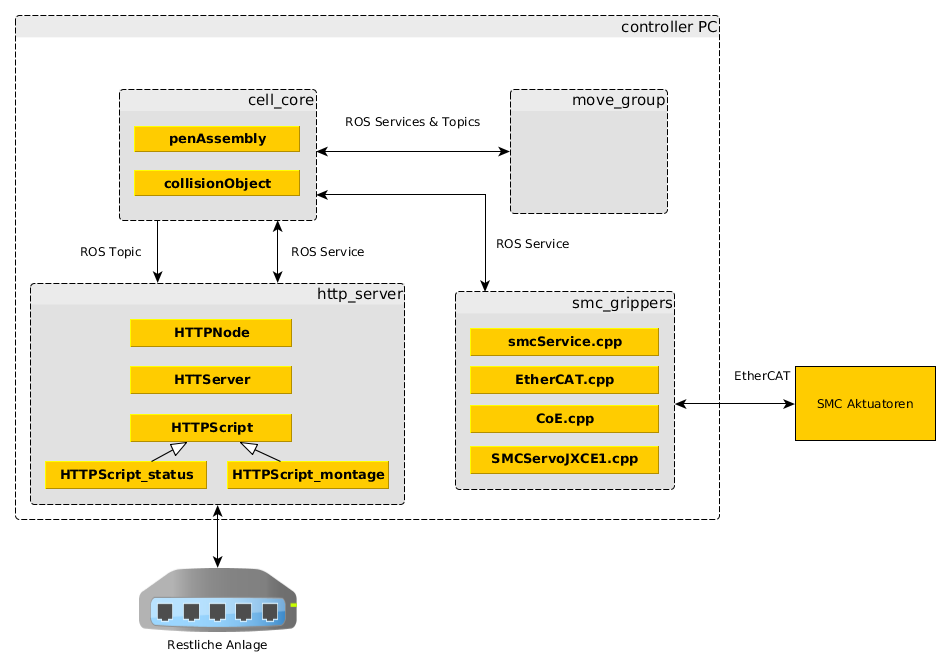
\includegraphics[width=0.95\textwidth]{uebersicht}
	\caption{Übersicht Packages und Kommunikation}
	\label{fig:Uebersicht}
\end{figure}

\section{cell\_core}
Das Package cell\_core ist das Kernelement der Implementierung von ROS. Das Package konstruiert die move\_group und kommuniziert anschliessend mit derselben um den momentan in der Anlage verbauten Roboter in Bewegung zu bringen. Das Package besteht aus einem Node 'penAssembly' und einer Klasse 'collisionAdder'. Das Package publiziert beim ROS-Master zwei Services und ein Topic, mit welchen es möglich ist mit dem Package zu kommunizieren.

\subsection{Topics}
Der Node publiziert regelmässig($10\;Hz$) den momentanen Anlagenstatus auf dem Topic /penAssembly/status. Die Publizierte Nachricht enthält die zwei booleschen Variablen idle und error. Welche je nach Zustand der Anlage gesetzt werden.

\subsection{Services}
Das Package cell\_core bietet zwei Services an, der erste Service startet den Zusammenbau eines Kugelschreibers. Der zweite Service ermöglicht es den Roboter an einen bestimmten Punkt und Orientierung zu bewegen.
\paragraph{moveRobotToPose}
Zum jetzigen Stand der Arbeit registriert sich bei diesem Service kein Node. Der Service wurde nur gebraucht um den Roboter über die Konsole mithilfe von\\
\mintinline{bash}{$ rosservice call /penAssembly/moveRobotToPose "x: ,y: ,z: ,oW: ,oX: ,oY : ,oZ: "} %$
zu einer bestimmten Position und Orientierung zu bewegen. Die Methode beachtet bei der Planung der Bewegung Kollisionsobjekte. Der Service Antwortet mit einem Boolean ob die Position erreicht wurde (true) oder nicht (false). Zum Aufrufen des Services müssen die Koordinaten sowie die Orientierung angegeben werden. Der Service ruft die Methode 'moveRobotCallback' auf.
\paragraph{montage\_service}
Der Service montage\_service ermöglicht es den Start der Montage auszulösen. Dabei muss der Nachricht der Offset der Wagen in Metern, sowie die gewünschte Ausgabestelle für den fertig montierten Kugelschreiber mitgegeben werden. Momentan ist die Ausgabe an verschiedene Stellen nur implementiert es existieren in der Anlage aber noch keine effektiven Ausgabestellen.
\begin{figure} [h!]
	\begin{minipage}[h]{0,49\textwidth}
		\begin{code}
			\begin{minted}{bash}
			#request
			float64 x
			float64 y
			float64 z
			float64 oW
			float64 oX
			float64 oY
			float64 oZ
			---
			#response
			bool status
			\end{minted}
			\vspace{-10pt}
			\caption{moveRobotToPose Message}
			\label{code:moveRobotMessage}
		\end{code}
	\end{minipage}
	\begin{minipage}[h]{0,49\textwidth}
		\begin{code}
			\begin{minted}{bash}
			#request
			float64 Offset
			int64 Ausgabestelle
			---
			#response
			int64 status			
			\end{minted}
			\vspace{-10pt}
			\caption{montage\_service Message}
			\label{code:montageMessage}
		\end{code}
	\end{minipage}
\end{figure}

\subsection{penAssembly} \label{sec:penAssembly}
\paragraph{Initialisierung}
Beim starten des penAssembly Nodes wird als erstes ROS initialisiert und anschliessend ein asynchroner Spinner gestartet. Der asynchrone Spinner ist nötig, damit bei aktiver Planung von Trajektorien andere Anfragen immer noch verarbeitet werden können. Anschliessend wird die move\_group gestartet und initialisiert, gefolgt vom Publizieren der beiden Services und des Topics. Als letztes wird ein Objekt der Klasse collisionObject erstellt und das Kollisionsobjekt der Anlage auf dem planning\_interface publiziert. Wenn dieses Setup durchgeführt wurde wechselt der Node in einen Endlosloop und publiziert mit einer Frequenz von $10\;Hz$ den Status der Anlage. Gleichzeitig wird auf den beiden publizierten Topics auf eine Anfrage gewartet.
\begin{code}
	\begin{minted}{cpp}
int main(int argc, char **argv)
{
	ros::init(argc, argv, "penAssembly");
	ros::NodeHandle nh;
	ros::AsyncSpinner spinner(0); // Define Multithreadedspinner
	spinner.start();

	// Define MoveGroup and PlanningSceneInterface
	group.reset(new moveit::planning_interface::MoveGroupInterface("gripper"));
	//group->setPlannerId("RRTConnect");
	group->setEndEffectorLink("grasping_frame");
	group->setPlanningTime(1.5);
	group->setGoalJointTolerance(0.0001);
	group->setNumPlanningAttempts(3);
	group->setGoalOrientationTolerance(0.0001);
	group->setMaxVelocityScalingFactor(0.1);

	// Advertise Services at ROS-Master
	ros::ServiceServer service = nh.advertiseService("/penAssembly/montage_service", montageCallback);
	ros::ServiceServer moveservice = nh.advertiseService("/penAssembly/moveRobotToPose", moveRobotCallback);
	ROS_INFO("Service rdy!");

	// Publish the Status updater
	ros::Publisher penAssembly_pub = nh.advertise<cell_core::status_msg>("/penAssembly/status", 1000);

	sleep(15); // to make sure move_group is up
	collisionObject coAdder;
	coAdder.addCell(group);
	sleep(10);	// only used because the large model takes some time to load

	ROS_INFO("Node Ready!");
	// Publish the State of the Assembly
	ros::Rate loop_rate(10); //Freq of 10 Hz
	while (ros::ok()) //aslong as node is alive
		{
			cell_core::status_msg msg;
			msg.idle = idle_;
			msg.error = error_;
			penAssembly_pub.publish(msg);
			loop_rate.sleep();
		}
}	
	\end{minted}
	\caption{Initialisierung penAssembly Node}
	\label{code:initPenAssembly}
\end{code}

\subsubsection{Methoden}
Der Node bietet mehrere Methoden, zwei der Methoden werden durch die Services aufgerufen, die restlichen Methoden werden durch diese beiden Callbackmethoden aufgerufen. Alle in penAssembly.cpp implementierten Methoden ermöglichen es dem Roboter sich auf eine bestimmte Art und Weise zu bewegen. 

\paragraph{montageCallback}
Die Methode montageCallback wird vom Service montage\_service aufgerufen. Die Methode überprüft zu Beginn, ob die mitgegebenen Werte korrekt sind und ob die Anlage sich im idle-Modus befindet. Falls die Kriterien erfüllt sind startet die Anlage die Montage eines Kugelschreibers, ansonsten wird kein Kugelschreiber montiert und ein Fehler zurückgegeben. Innerhalb der Methode ist der Ablauf für die Montage des Kugelschreibers definiert. Der Roboter fährt jeweils mit freier Trajektorienplanung an ein Offset Punkt vor der eigentlichen Pose. Anschliessend wird der restliche Weg mit einem linearen Fahrbefehl gefahren. 

\paragraph{initPoses}
Die Methode init Poses wird bei jedem Start eines Montage Prozesses aufgerufen, diese Initialisiert alle für die Montage benötigten Posen des Roboters. Ihr wird der Offset aus dem Servicecall mitgegeben, damit die Position des Schlittens korrigiert werden kann.

\paragraph{moveLinear}
Diese Methode bewegt den Roboter auf einer geraden Linie zwischen zwei Punkten. Der Startpunkt entspricht dabei immer der momentanen Position des Roboters, als Endpunkt kann entweder der Fahrweg von Startpunkt zu Zielpunkt in Metern in x,y,z mitgegeben werden, oder eine Pose zu welcher gefahren werden soll. Die Methode benötigt zudem den Plan des MoveGroupInterfaces.
Die Trajektorie zwischen dem Start- und Endpunkt wird mithilfe der Methode computeCartesianPath berechnet, welche Teil der move\_group ist. Der Trajektorie wird nur ausgeführt, falls der Planner mehr als 90\;\% des vorgegebenen Weges einhalten kann. Falls dies der Fall ist gibt die Methode true zurück.
\begin{code}
	\begin{minted}{cpp}
bool moveLinear(double x, double y, double z, moveit::planning_interface::MoveGroupInterface::Plan &plan)
{
    std::vector<geometry_msgs::Pose> waypoints_tool;
    // Getting the current pose
    geometry_msgs::PoseStamped tempStampPose = group->getCurrentPose(group->getEndEffectorLink());
    geometry_msgs::Pose test_pose = tempStampPose.pose;
	// Defining Endpose
    test_pose.position.x += x;
    test_pose.position.y += y;
    test_pose.position.z += z;
    waypoints_tool.push_back(test_pose);

    moveit_msgs::RobotTrajectory trajectory_msg;
    double fraction = group->computeCartesianPath(waypoints_tool,
                                                  0.001, //eef_step
                                                  5,     // jump_threshold
                                                  trajectory_msg, 
                                                  true); //avoid collisions
    plan.trajectory_ = trajectory_msg;
    ROS_INFO("Visualizing Cartesian Path (%2f%% acheived)", fraction * 100.0);
    if (fraction >= 0.90)
    {
        group->execute(plan);
        return 1;
    }
    else
    {
        return 0;
    }
    return -1;
}
	
	\end{minted}
	\vspace{-10pt}
	\caption{moveLinear mit x,y,z Offset}
	\label{code:moveLinear}
\end{code}

\paragraph{movePen}
Die Methode movePen wird gebraucht um den Kugelschreiber von der 45\;\textdegree Lage in die Senkrechte Position aufzurichten. 

\paragraph{rotateZ}
Die Methode rotateZ wird aufgerufen um den Kugelschreiber mit dem Werkzeuge auszurichten. Sie ist die einzige Methode, welche anstatt auf Positionen zu Planen direkt auf Gelenkwinkel plant. Der Methode muss ein Winkel in Radiant mitgegeben werden, um welchen sich die sechste Achse in positiver Richtung drehen soll.
\begin{code}
	\begin{minted}[breakanywhere]{cpp}
void rotateZ(moveit::planning_interface::MoveGroupInterface::Plan &plan, double angle)
{
	std::vector<double> group_variable_values;
	// Saves the current Joint values in the vector group_variable_values
	group->getCurrentState()->copyJointGroupPositions(group->getCurrentState()->getRobotModel()->getJointModelGroup(group->getName()), group_variable_values);
	// Defining goal JointValue of joint6
	group_variable_values[5] += angle;
	group->setJointValueTarget(group_variable_values);
	// plan and execute
	group->plan(plan);
	group->execute(plan);
}
	\end{minted}
\vspace{-10pt}
\caption{Methode rotateZ}
\label{code:methRotz}
\end{code}

\paragraph{moveToPose}
Die Methode moveToPose bewegt den Roboter an die angegebene Pose, es ist möglich der Methode einen Offset in x,y und z mitzugeben. Falls der Planer beim ersten versuch keine Lösung findet wird die Planungszeit auf $10\;s$ erhöht und ein neuer Planungsversuch gestartet. Falls immer noch keine Lösung für die Bewegung gefunden wird gibt die Methode false zurück.

\subsection{collisionAdder}
Die Klasse collisionAdder ermögtlicht es Kollisionsobjekte in die Planungsszene zu laden, dazu bietet sie vier Methoden an.
\paragraph{addCell} Die Methode addCell wird kurz nach dem erstellen des Objekts beim Initialisieren des Nodes aufgerufen. Sie fügt der Planungsszene das Kollisionsmodell der Anlage hinzu, welches direkt aus dem .stl-File generiert wird. 
\begin{code}
	\begin{minted}{cpp}
void collisionObject::addCell(boost::shared_ptr<moveit::planning_interface::MoveGroupInterface> &group)
{
    // Generating Collision object from Mesh
    Eigen::Vector3d scaling_vector(0.001, 0.001, 0.001); // Scaling Vector
    moveit_msgs::CollisionObject co;
    co.header.frame_id = group->getPlanningFrame();
    co.id = "WorkCell";
    shapes::Mesh *m = shapes::createMeshFromResource("package://cell_support/meshes/1000_Anlage_collision.stl", scaling_vector);
    ROS_INFO("Mesh Loaded");

    shape_msgs::Mesh mesh;
    shapes::ShapeMsg mesh_msg;
    shapes::constructMsgFromShape(m, mesh_msg);
    mesh = boost::get<shape_msgs::Mesh>(mesh_msg);

    // Define position and orientation
    co.meshes.resize(1);
    co.mesh_poses.resize(1);
    co.meshes[0] = mesh;
    co.mesh_poses[0].position.x = -1.075;
    co.mesh_poses[0].position.y = 0.023;
    co.mesh_poses[0].position.z = -0.021;
    co.mesh_poses[0].orientation.w = 0.707;
    co.mesh_poses[0].orientation.x = 0.0;
    co.mesh_poses[0].orientation.y = 0.0;
    co.mesh_poses[0].orientation.z = 0.707;

    // Push onto vector and publish it on the szene
    co.meshes.push_back(mesh);
    co.mesh_poses.push_back(co.mesh_poses[0]);
    co.operation = co.ADD;
    std::vector<moveit_msgs::CollisionObject> collision_objects;
    collision_objects.push_back(co);
    planning_scene_interface.addCollisionObjects(collision_objects);
    return;
}

	\end{minted}
\vspace{-10pt}
\caption{addCell Methode}
\label{code:addCell}
\end{code}

\paragraph{addBody}
Die Methode addBody publiziert einen Kollisionskörper am momentan aktiven Planningframe des Roboters und befestigt diesen direkt daran. Die Methode besitzt ein Switchstatement, welches einen Übergabewert auswertet. Mit diesem kann zwischen der vorderen Hülle (1) dem Deckel (2), der Miene (3) und dem Werkzeug (4) ausgewählt werden. Die Kollisionskörper werden wie bei der Methode addCell direkt aus den .stl-Files der Teile erstellt. 

\paragraph{detatchBody}
Diese Methode entfernt ein zuvor publiziertes Kollisonsobjekt vom Roboter, entfernt es jedoch noch nicht aus der Plannungsumgebung. Auch hier können die Objekte wieder über den übergebenen Integer ausgewählt werden.

\paragraph{removeBody}
Die Methode entfernt ein sich in der Planungsszene befindendes Objekt ganz. Die Methode benötigt die selben Übergabewerte wie die beiden vorhergegangenen Methoden.

\subsection{launch}
Das Package enthält zwei launch-Files, das Erste startet alle benötigten Nodes für den Industriedemonstrator, verbindet sich aber nicht mit einem angeschlossenen Roboter. Das andere .launch-File startet auch alle benötigten Nodes, versucht aber zudem eine Verbindung mit dem angeschlossenen Roboter herzustellen (momentan ABB IRB120).
Es wurden auch launch-files für den Stäubliroboter generiert, bei diesen konnte jedoch nicht getestet werden ob sie eine Verbindung mit dem Roboter herstellen, da der Roboter noch nicht geliefert wurde.

\section{http\_server}
Der HTTP-Server basiert auf dem im SVN-Repository \url{https://triest.zhaw.ch/svn/iio/} vorhandenen Sourcecode. Es wurde zusätzlich ein ROS Node erstellt, welcher die für den Betrieb des HTTP-Servers nötigen Objekte generiert. Der Node erstellt zwei unterschiedliche Server auf den Ports 8080 und 8081, auf dem Port 8080 kann die Montage eines Kugelschreibers ausgelöst werden. Dazu muss die folgende URL mit den entsprechenden Werten aufgerufen werden:\\
\url{http://160.85.95.166:8080/cgi-bin/montage?offset=0.0\&ausgabestelle=1}\\
Der Offset muss in Metern angegeben werden wobei positive Zahlen einen Offset in Fahrtrichtung der Wagen entsprechen.\\

Mit dem Webserver auf Port 8081 kann der Status des Roboters abgefragt werden, dazu kann die folgende URL aufgerufen werden:\\
\url{http://160.85.95.166:8080/cgi-bin/status}

Bei beiden Aufrufen ist allenfalls die IP-Adresse zu ändern.

\begin{code}
	\begin{minted}{cpp}
#include <http_server/HTTPNode.h>

int main(int argc, char **argv)
{
    ros::init(argc, argv, "HTTP_server");
    ros::NodeHandle nh;
    ros::AsyncSpinner spinner(2); // Define Multithreadedspinner
    spinner.start();

    HTTPServer *httpServer = new HTTPServer(8080);
    HTTPServer *httpServer2 = new HTTPServer(8081);
    httpServer->start();
    httpServer2->start();
    httpServer->add("montage", new HTTPScript_montage());
    httpServer2->add("status", new HTTPScript_status());

    ROS_INFO("Http-Server is running!");

    ros::waitForShutdown();
}
	\end{minted}
\vspace{-10pt}
\caption{Main des HTTP-Servers}
\label{code:httpMain}
\end{code}
\subsection{launch}
Der Webserver kann über das launch-File 'httpNode.launch' gestartet werden, das launchfile Startet im falle eines Absturzes des HTTP-Nodes diesen direkt neu.

\section{smc\_grippers}
Die Controller für die SMC Aktuatoren müssen über EtherCAT angesteuert werden. Durch die ROS Community sind einige Packages vorhanden, welche dazu gedacht sind EtherCAT Geräte anzusteuern. Diese basieren in der Regel entweder auf dem \gls{SOEM} der OpenEtherCAT Society, oder auf dem EtherCAT Treiber des PR2 von Willow Garage. Es wurde mit mehreren dieser verfügbaren Packete versucht eine erfolgreiche Kommunikation mit den EtherCAT Kontrollern von SMC aufzubauen. Diese Versuche blieben jedoch erfolglos. Aus diesem Grund wurde durch Herrn Dr. Marcel Honegger ein Treiber für die EtherCAT Kontroller von SMC geschrieben. Diese Sourefiles wurden anschliessend in ein ROS Node eingebunden, welcher für jeden Aktuator von SMC einen eigenen Service anbietet.\\
\begin{code}
	\begin{minted}{cpp}
bool smcService::gripperCallback(smc_grippers::gripper_service::Request &req, smc_grippers::gripper_service::Response &res)
{
    gripper->enable();
    int pos = req.position;
    gripper->setTargetPosition(pos);
    gripper->disable();
    return 1;
}
	\end{minted}
\vspace{-10pt}
\caption{Callbackmethode des Greifers}
\label{code:CallbackGripper}
\end{code}

Im momentanen Stand der Anlage ist noch keine Kommunikation mit den Kontrollern von SMC möglich, da es vom Linux PC nicht möglich ist, dass die Slaves in den EtherCAT status Operational wechseln. 

\subsection{Services} %TODO: Services anpassen und SMC Teil programmieren.
Die drei Services sind identisch aufgebaut und benötigen alle nur die gewünschte Position in Millimeter. Die Services antworten immer mit true, ausser die Services sind nicht erreichbar.

\subsection{launch}
Der SMC Node kann mithife des launch-File 'smcService.launch' gestartet werden.

